\documentclass{article}
\usepackage{graphicx}
\usepackage{float}
\usepackage[table]{xcolor}
\usepackage{amsmath}
\usepackage{booktabs}
\usepackage{caption}
\usepackage{geometry}
\usepackage{array}
\usepackage{tabularx}
\usepackage{hyperref}
\usepackage[nottoc,numbib]{tocbibind}
\usepackage[titletoc,toc,page]{appendix}
\addtocontents{toc}{\protect\thispagestyle{empty}}

\geometry{a4paper, margin=1in}
\definecolor{TikTokBlack}{HTML}{040404}
\definecolor{TikTokPink}{HTML}{de8c9d}
\definecolor{TikTokRed}{HTML}{fe2858}
\definecolor{TikTokLightBlue}{HTML}{2af0ea}
\definecolor{TikTokDarkBlue}{HTML}{397684}

\begin{document}

% Center everything on the page
\begin{titlepage}
\begin{center}

    % Logo and title
    
\includegraphics[width=0.1\textwidth]{./resources/logo.png} \\
    \vspace{0.5cm}
    {\Huge \textbf{TikTok-Brain}} \\[0.5cm]
    {\LARGE \textit{Lo-fi Prototyping and Usability Testing}} \\[2cm]

\end{center}

    % Mission Statement
    \noindent
    \textbf{\textcolor{TikTokLightBlue}{\Large Mission Statement}} \\[0.3cm]
    \parbox{\textwidth}{
        \large
        To promote stair safety by leveraging the captivating power of video,
        delivering crucial safety messages in an engaging and distraction-free platform.
        % TikTok-Brain is both a community and competition platform that empowers individuals to take sustainable actions.
    } \\[1cm]

    % Value Proposition
    \noindent
    \textbf{\textcolor{TikTokBlack}{\Large Value Proposition}} \\[0.3cm]
    \parbox{\textwidth}{
        \large
        % Teamwork makes the green work.
        Delivering mesmerizing, randomized videos paired with essential safety advisories,
        TikTok-Brain simplifies social media to focus solely on enhancing personal safety without the clutter of likes, comments, or shares.
    } \\[1cm]


    % Problem / Solution Overview
    \noindent
    \textbf{\textcolor{TikTokRed}{\Large Problem / Solution Overview}} \\[0.3cm]
    \parbox{\textwidth}{
        \large
        Many individuals are unaware of the risks associated with inattentive stair use.
        Traditional safety messages often fail to engage audiences, leading to continued accidents and injuries.
        TikTok-Brain combines the engaging nature of short-form video content with critical safety messaging.
        By removing typical social media distractions,
        the app ensures that users receive and retain important information about walking safely on stairs.
    } \\[1.5cm]

\begin{center}
    % Our Team
    \textbf{\textcolor{TikTokBlack}{\Large Our Team}} \\[0.5cm]

    % Team Photos and Names
    \begin{tabular}{ccc}
        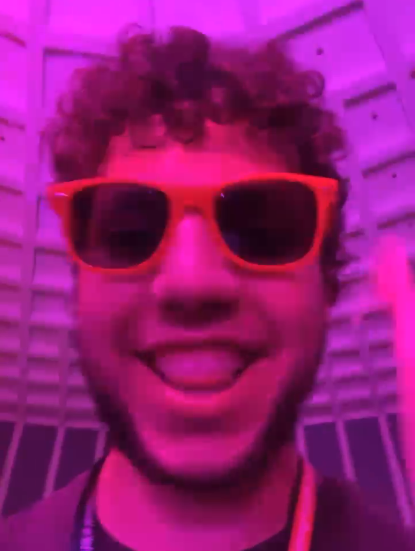
\includegraphics[width=0.2\textwidth]{./resources/ole.png} &
        
\includegraphics[width=0.2\textwidth]{./resources/markus.png} &
        
\includegraphics[width=0.2\textwidth]{./resources/diba.png} \\[0.3cm]
        Ole Einar Grundmann & Markus Siegert & Diba Zokai \\
    \end{tabular}
\end{center}
\end{titlepage}

\newpage
\tableofcontents
\newpage

\section{Introduction}
% Provide an introduction to the project, discussing the background, motivation, and objectives of your work. Describe the problem in more detail and explain why sustainability is crucial.
Distracted walking has become a significant safety concern, particularly on stairs where attention is crucial.
Traditional social media platforms, designed for high engagement,
inadvertently increase these risks by encouraging users to focus more on their screens than their surroundings.

TikTok-Brain is designed to counteract this issue by combining the engaging nature of video content
with crucial safety messages about walking safely on stairs.
This app simplifies the social media model: it removes likes, comments, and shares,
focusing solely on delivering safety-oriented content through mesmerizing, randomized videos paired with safety advisories.

\section{Methodology}
% This section explains the methodology used in your project. Break it down into subsections for clarity.
The process began with an individual brainstorming phase,
where each team member independently generated ideas.
These ideas were then collectively refined using digital tools such as LaTeX, Gimp, and Krita,
resulting in a diverse array of 25 to 30 potential concepts.

To ensure our ideas were aligned with user needs and expectations,
we proceeded to create and conduct a detailed interview comprising 20 questions,
which was administered to 30 participants using Telekom Vote 2 and WhatsApp to reach out to the participants.
The insights gathered during these interviews were crucial. They helped constructing personas and refine our initial ideas.

With a solid understanding of our user base,
we evaluated the brainstormed ideas through a structured pro-contra analysis,
taking into account the feedback and personas developed earlier.
This phase of assessment was supported by Google Docs and LaTeX,
allowing us to narrow down our options to three final ideas.

Subsequently, we moved to visually conceptualize these ideas through sketches and storyboards,
utilizing Gimp, other graphic tools, and Kdenlive.
This step was vital in visualizing the sequence and flow of interactions,
which were crucial for the later stages of prototyping.

This iterative process of development and refinement led to the selection
of the most promising prototype based on its functionality and user feedback.

The final stage of our project involved the creation of professional presentations and a comprehensive final report,
crafted using PowerPoint and LaTeX. These documents provided a detailed overview of the project process,
from the initial concept to the final evaluation of the prototype.
This ensured that every aspect of the project was clearly documented.

\section{Results}

\subsection{Concept Sketches}
All our sketches and results here
\begin{table}[H]
\centering
\renewcommand{\arraystretch}{1.5}
\setlength{\tabcolsep}{12pt}
% \captionsetup{labelformat=empty}
% \caption{Figure 8: Pro + Con analysis for rewards interface}
    \begin{tabularx}{\textwidth}{|>{\centering\arraybackslash}X|>{\centering\arraybackslash}X|}
\hline
        \cellcolor{TikTokRed}\textbf{Pros} & \cellcolor{TikTokLightBlue}\textbf{Cons} \\ \hline
Graphic showing saving accumulation encourages long term behavior change & Individualized rewards might not be as fulfilling as team rewards \\ \hline
Gives users information about where they can spend their rewards & Focus on monetary rewards may discourage users \\ \hline
Small but steady rewards encourage the user to continue returning to the app & Plus / Minus button could be frustrating to use \\ \hline
\end{tabularx}
\end{table}

\subsection{Prototyping}
% Present the results of your project in this section. You might want to use tables, charts, and figures to show the data clearly.
% Explain the process of creating the low-fidelity prototype. Include diagrams or wireframes if available:

\begin{table}[H]
\centering
\renewcommand{\arraystretch}{1.5}
\setlength{\tabcolsep}{12pt}
    \begin{tabularx}{\textwidth}{|l|X|X|}
        \hline
        \cellcolor{TikTokRed}\textbf{Component} & \cellcolor{TikTokBlack}\textbf{\textcolor{white}{Description}} & \cellcolor{TikTokLightBlue}\textbf{Functionality} \\
        \hline
        Video Display Area & Fullscreen area to show videos. & Displays a single video at a time, taking up the bottom part of the screen. \\
        \hline
        Swipe Navigation & Gesture-based navigation for moving through videos. & Swiping up loads the next video; swiping down loads the previous video, if available. \\
        \hline
        Random Video Loader & Logic that fetches a random video to display. & Randomly selects and loads a video from the video pool whenever a new video is required (e.g., after reaching the end of history). \\
        \hline
        Text Overlay Area & Area at the top of the screen for text that accompanies each video. & Displays a random line of text (e.g., a phrase or quote) that’s paired with the video. \\
        \hline
        Reload Mechanism & Mechanism to refresh the video feed if there are no previous videos in history. & Reloads the video feed to pull a new batch of random videos when the user reaches the top of the stack. \\
        \hline
        Video-Text Randomizer & Logic that pairs random videos with random text. & Ensures that each video is matched with a different text overlay each time it appears, maintaining freshness. \\
        \hline
        Interface Background & Background color or visual design behind the video display. & Provides visual consistency or mood but stays unobtrusive to keep focus on video and text content. \\
        \hline
        Loading Indicator & Small icon or animation that shows when new content is being loaded. & Briefly appears when the app fetches a new random video or reloads the feed. \\
        \hline
        No Interaction Buttons & No buttons for like, comment, or share, emphasizing simplicity. & Only swipe gestures are recognized; no additional UI elements for social interactions. \\
        \hline
        Error Handling Display & Fallback message or visual when loading fails. & Displays an error message if a video fails to load, with a prompt to swipe to reload. \\
        \hline
        Auto Swipe Animation & Animation that mimics a swipe if there’s no interaction for a while. & After a set period of inactivity, automatically performs a swipe animation to move to the next video, keeping the experience engaging. \\
        \hline
    \end{tabularx}
    \caption{Functionality of Design Interface Components}
\end{table}

\begin{figure}[H]
    \centering
    \includegraphics[width=0.8\textwidth]{prototype.png} % Replace with path to prototype image
    \caption{Lo-fi Prototype of TikTok-Brain Platform}
    \label{fig:prototype}
\end{figure}

\begin{table}[H]
    \centering
    \begin{tabular}{|c|c|c|}
        \hline
        Metric & Prototype & Feedback Score \\
        \hline
        Usability & 4.5 & Positive \\
        Sustainability Awareness & 4.2 & Neutral \\
        Engagement & 4.8 & Very Positive \\
        \hline
    \end{tabular}
    \caption{Usability Testing Results}
    \label{tab:results}
\end{table}

\section{Discussion}
Analyze the results here, discussing what the results imply about the effectiveness of your platform. Discuss any limitations or challenges encountered.

\section{Conclusion}
Summarize the key findings and discuss the impact of your work. Outline potential future work or improvements for the platform.

\newpage
\bibliographystyle{ieeetr}
\bibliography{Bibliography}
\newpage

\renewcommand{\thesection}{\Alph{section}}

\appendix

\section{AI Appendix}
asdf

\end{document}
